% 2. Отображение предметной области на многоуровневые архитектуры

\chapter{Отображение предметной области на многоуровневые архитектуры}

Разработка больших программ – многоступенчатый процесс, в ходе которого осуществляются как ручные трансформации неформальных моделей решаемой задачи в формализованные представления, так и их последующая автоматическая трансформация с использованием различных систем программирования.

\begin{itemize}
    \item Предметная область
    \item Архитектура ВС
    \item Инструменты для разработки ПО
\end{itemize}

\begin{figure}[htbp]
    \centering
    
\includegraphics[width=0.8\textwidth]{img/reflection-02.png}
    \caption{Три кита, определяющие процесс разработки программ}
    \label{reflection-02}
\end{figure}

\section{Влияние особенностей архитектур вычислительных систем («железо», ОС, ЯП)}

\begin{itemize}
    \item время выполнения программы
    \item особенности программирования
    \item особенности оборудования
    \item …
\end{itemize}

Помимо увязки моделей предметной области с архитектурой ВС, встают проблемы, определяемые спецификой инструментов, используемых для создания программ.

Можно выделить технологическое направление, напрямую не связанное с предметной областью.

В его рамках формулируются требования:

\begin{itemize}
    \item к средствам, обеспечивающим написание программ,
    \item к средствам проектирования, определяющим переход от моделей предметной области к программам.
\end{itemize}

Огромную роль на разработку ПО оказывает необходимость соответствия заданным критериям качества.
Ряд критериев вытекает из особенностей предметной области. Другие обуславливаются архитектурой ВС и другими причинами.

\textbf{Вместе они характеризуют комплекс проблем, преодолеть который пытаются разработчики программного обеспечения.}

\section{Критерии качества программного обеспечения}

Применение информационных технологий немыслимо без создания программного обеспечения (ПО), разработка которого зачастую является сложным многоступенчатым процессом. Существуют альтернативные взгляды на этот процесс. Но в целом он связан с построением различных моделей, начиная от моделей предметной области и заканчивая моделями, воплощенными в законченном программном продукте. При этом осуществляются ручные трансформации неформального представления предметной области, определяющего понятия решаемой задачи, в ее формализованное представление. Полученные модели описываются в виде программ на языках программирования, после чего происходит их трансформация в машинные коды. Предметная область во многом определяет специфику разрабатываемых приложений, характеризуя состав и особенности используемых моделей, создание которых бывает весьма сложным и многогранным. Их окончательная структура может формироваться не только во время написания программы, но и в ходе ее выполнения за счет динамического связывания.

В немалой степени на процесс программирования влияют также особенности компьютеров, недооценка которых может привести к резкому снижению эффективности процесса обработки данных. Это обуславливается нюансами их внутренней организации, ориентацией на различные предметные области, и проявляется для программистов через компьютерную архитектуру, а также языки и системы программирования.

Наряду с необходимостью увязки моделей предметных областей и архитектур вычислительных систем, перед программистами встают проблемы, решение которых определяется спецификой инструментов, используемых для создания программ. Попытки решить их привели к выделению технологического направления, напрямую не связанного с предметной областью. В его рамках формулируются требования как к средствам кодирования, обеспечивающим написание программ, так и к средствам проектирования, определяющим переход от моделей предметной области к программам.

Между системами программирования и методами разработки ПО нет четкой грани. Существует их взаимное влияние друг на друга вне зависимости от используемых подходов и технических средств. Совместное использование заключается в том, что методы проектирования применяются для «ручного» перехода от исходных моделей к программам, а системы программирования обеспечивают непосредственное написание программ и их автоматический перевод в язык конкретного исполнителя. Например, объектно-ориентированная методология (ООМ) предлагает унифицированный процесс проектирования, инструментальная поддержка которого обеспечивает непосредственное построение каркасов программных приложений. Совместное использование методик проектирования и систем программирования осуществляется также при других методах разработки программного обеспечения.

В рамках технологии программирования проводятся исследования методов разработки, обеспечивающих создание продуктов, соответствующих заданным критериям качества. Ряд этих критериев вытекает из особенностей построения моделей предметной области. Другие обуславливаются сугубо внутренними причинами. Вместе они характеризуют комплекс проблем, преодолеть который пытаются разработчики систем программирования. Некоторые из критериев учитывают правила конструирования и технику написания программы. В частности, к ним относятся:

\begin{itemize}
    \item Корректность (правильность). Программа обеспечивает правильную обработку на правильных данных.
    \item Устойчивость. Программа «элегантно» завершает обработку ошибок.
    \item Расширяемость. Программа может легко адаптироваться к изменяющимся требованиям.
    \item Многократность использования. Программа может использоваться и в других системах, а не только в той, для которой было создана.
    \item Совместимость. Программа может легко использоваться с другим программным обеспечением.
    \item Эффективность. Обеспечивается эффективное использование времени, компьютерной памяти, дискового пространства и т.д.
    \item Переносимость. Разработанное программное обеспечение можно легко перенести на другие аппаратные и программные средства.
    \item Верификация. Простота проверки, легкость разработки тестов при обнаружении ошибок, легкость обнаружения мест, где программа потерпела неудачу, и т.д.
    \item Поддержка целостности. Программа защищает себя от неправильного обращения и неправильного употребления.
    \item Легкость использования. Не возникает проблем для пользователя в эксплуатации программы, а для будущих программистов в ее дальнейшем сопровождении и развитии.
\end{itemize}

Невозможно сопоставить важность указанных характеристик, так как все они, в той или иной степени, должны учитываться при разработке программного обеспечения. Вместе с тем следует отметить их относительную независимость, что позволяет сконцентрировать исследования на более тщательной проработке отдельных компонент перспективных систем программирования, отвечающих за конкретные критерии качества.

Не следует пренебрегать и организационными аспектами процесса разработки ПО, определяющими построение коллектива разработчиков, распределение ролей на выполнение различных видов работ. Это один из существенных факторов, во многом определяющих успешность создания требуемого программного продукта. Именно вокруг того, как организовать работу над программным проектом постоянно идут оживленные дискусси и ломаются копья. Однако в данном материале я не буду заострять внимание на этом важном с точки зрения реального проектирования вопросе, акцентировав основное внимание на технической, а не организационной стороне.

\subsection{Факторы, определяющие процесс разработки программного обеспечения}

Среди множества факторов, от которых зависит процесс разработки программного обеспечения, можно выделить:

\begin{itemize}
    \item классы решаемых, задач, определяющие смысловое содержание создаваемых программ;
    \item методологии, задающие особенности организационного и технического проведения основных этапов разработки программного обеспечения;
    \item методы и парадигмы программирования, обуславливающих стили кодирования и архитектуры виртуальных машин;
    \item аппаратные и системные программные средства, предоставляющие виртуальные и физические ресурсы для непосредственного использования ПО.
\end{itemize}


Разнообразие этих факторов определяет множество вариантов, связанных с организацией процесса разработки. Определим его основные составляющие.

Цель процесса разработки – создание программы, обеспечивающей решение поставленной задачи некоторым исполнителем и удовлетворяющей при этом требуемым критериям качества. Решаемая задача описывается совокупностью формальных и эмпирических (неформальных) моделей, определяющих как протекающие в программе процессы, так и используемые при этом данные.

Модель задачи – совокупность специализированных моделей, описывающих различные аспекты решаемой задачи, отражаемые в разрабатываемой программе.

Специализированная модель – модель, предназначенная для описания определенных параметров рассматриваемого явления. Используется для акцентирования внимания на частных характеристиках.

Разрабатываемая программа должна обеспечивать выполнение функций, необходимых для решения задачи, в соответствующем исполнителе (вычислительной системе), специфика которого отражается в его модели.

Модель исполнителя – совокупность специализированных моделей, описывающих организацию и поведение вычислительной системы, осуществляющей выполнение программы.

Создаваемая программа является отображением модели решаемой задачи на модель исполнителя. Общая схема этого процесса разработки представлена на рисунке~\ref{fig01-01}. Трудоемкость программирования, с одной стороны, определяется количеством специализированных моделей, описывающих задачу, их размером, семантическим отличием от специализированных моделей исполнителя. С другой стороны она зависит от характеристик модели исполнителя, задающей требования к уровню абстракции разрабатываемой программы и ее приближенностью к архитектуре реального вычислителя.

\begin{figure}[htbp]
    \centering
    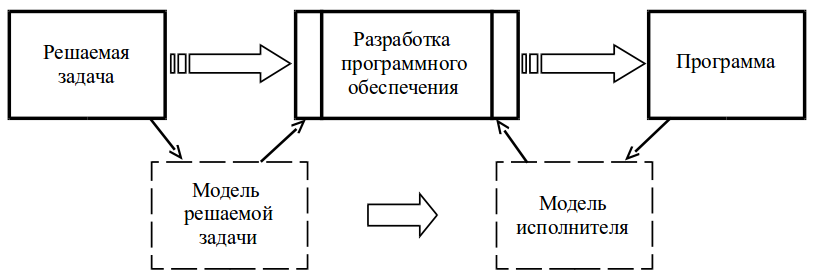
\includegraphics[width=0.9\textwidth]{img/fig01-01.png}
    \caption[Процесс разработки ПО]{Процесс разработки программного обеспечения как отображение модели задачи на модель исполнителя}
    \label{fig01-01}
\end{figure}

Сложность модели задачи может потребовать ее поэтапного преобразования в модель исполнителя, что схематически представлено на рисунке~\ref{fig01-02}. Необходимость в подобных преобразованиях обуславливается наличием семантического разрыва между моделями задач и исполнителей. Он проявляется в том, что объекты и операции, которыми разработчик манипулирует при описании задачи, не совпадают с объектами и операциями, используемыми при построении программы. Преодоление семантического разрыва осуществляется использованием методических и технических приемов, повышающих, к тому же, эффективность процесса разработки ПО.

\begin{figure}[htbp]
    \centering
    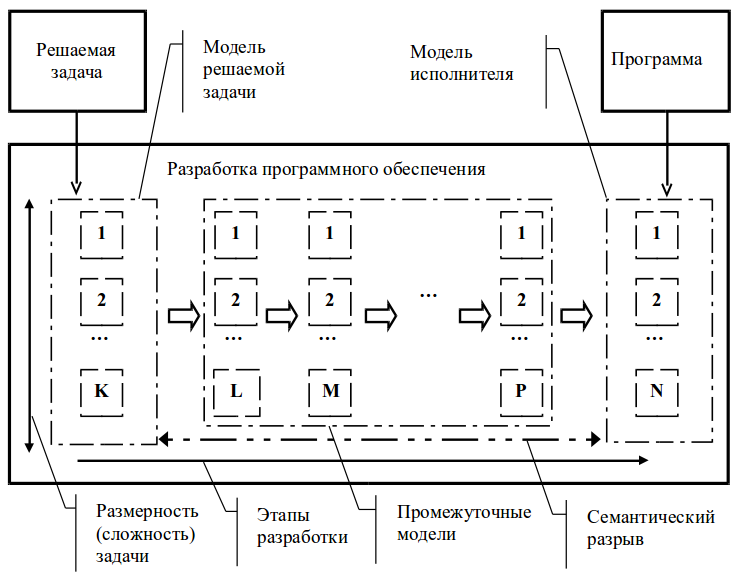
\includegraphics[width=0.9\textwidth]{img/fig01-02.png}
    \caption[Сложность преобразования моделей]{Влияние сложности задачи на процесс преобразования исходных моделей в модели исполнителя}
    \label{fig01-02}
\end{figure}

Разбиение моделей по различным этапам позволяет оценить объем работ на каждом из них. Помимо этого можно получить и временные характеристики как для каждого этапа, так и для всего процесса разработки ПО в целом. Общий объем работ определяется суммарным объемом, связанным с построением всех специализированных моделей. Условно это представлено на рисунке~\ref{fdiag01}.

\begin{figure}[htbp]
    \centering
    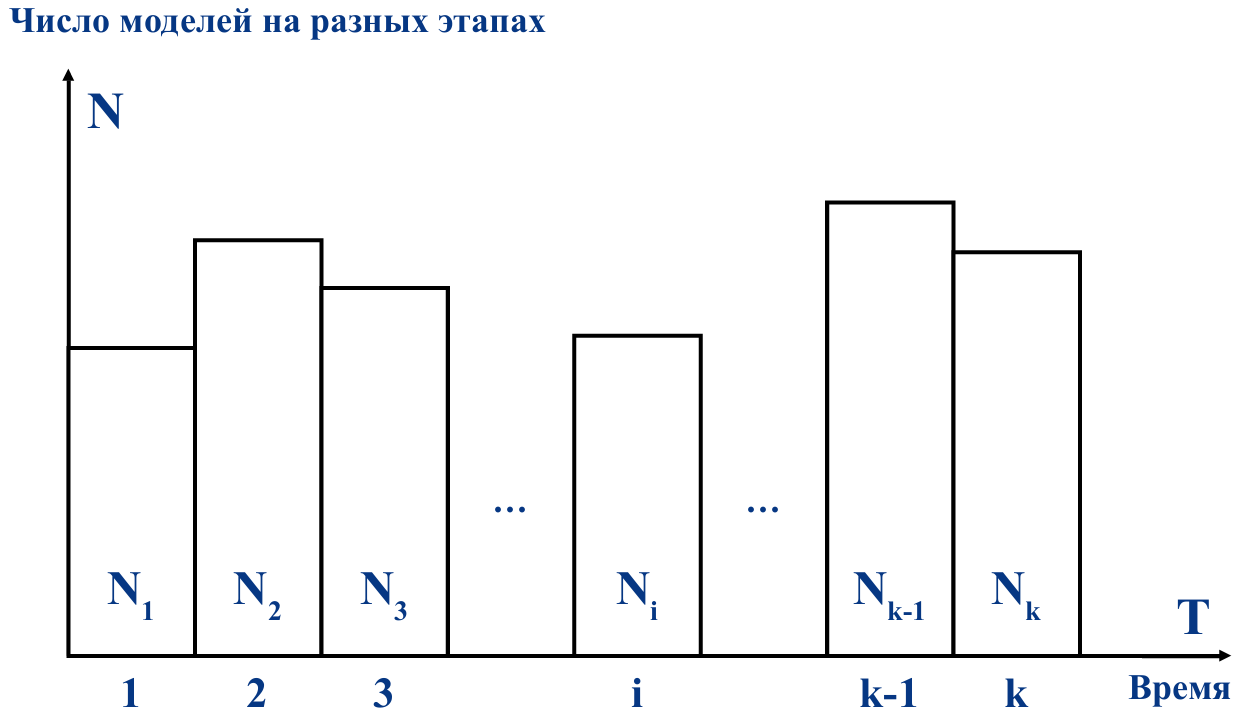
\includegraphics[width=0.9\textwidth]{img/fdiag01.png}
    \caption{Отображение объема работ и времени их выполнения в ходе разработки ПО}
    \label{fdiag01}
\end{figure}

\subsection{Методические приемы}

\textbf{Методические приемы} ориентированы на формализацию представления моделей и методов перехода между ними. Они позволяют ускорить процесс разработки следующими способами:

\begin{itemize}
    \item формализацией предметных областей;
    \item созданием методик разработки программного обеспечения.
\end{itemize}

\subsubsection*{Формализация предметной области}

Формализация предметной области заключается в построении ее модели и разработке методов преобразования модели предметной области в модель исполнителя. Модель предметной области объединяет совокупность специализированных моделей предназначенных для описания определенного класса решаемых задач, что обеспечивают ограничения на формируемое решение сверху. Дальнейший переход к модели исполнителя обычно осуществляется по выработанным методам или алгоритмам (рисунок~\ref{fig01-03a}).

\begin{figure}[htbp]
    \centering
    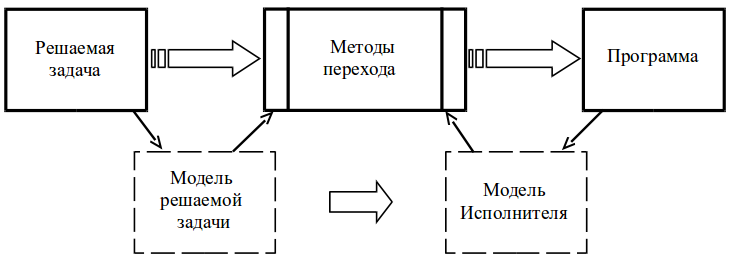
\includegraphics[width=0.9\textwidth]{img/fig01-03a.png}
    \caption{Формализация предметной области за счет разработки методов перехода от модели решаемой задачи к программе}
    \label{fig01-03a}
\end{figure}

Подобный подход широко используется при разработке программ в разных предметных областях. В качестве примеров, можно привести:

Построение синтаксических и лексических анализаторов. Модель предметной области, то есть язык программирования, описывается с использованием формальных грамматик, определяющих принципы порождения правильных цепочек языка. Наличие эквивалентности между различными грамматиками и автоматами позволяет перейти к распознавателям цепочек путем использования наработанных методов их программной реализации.

Разработка программных систем на основе теории автоматов, например, автоматное программирование. Последующая программная реализация автоматов является хорошо отработанным формальным приемом с применением различных технологий.

Основной эффект достигается за счет того, что при проработке и/или формализации методов используются уже полученные знания, что позволяет ускорить построение требуемых моделей. Это, в свою очередь, сокращает общий объем выполняемых работ и время выполнения процесса разработки (рисунок~\ref{fdiag02}).

\begin{figure}[htbp]
    \centering
    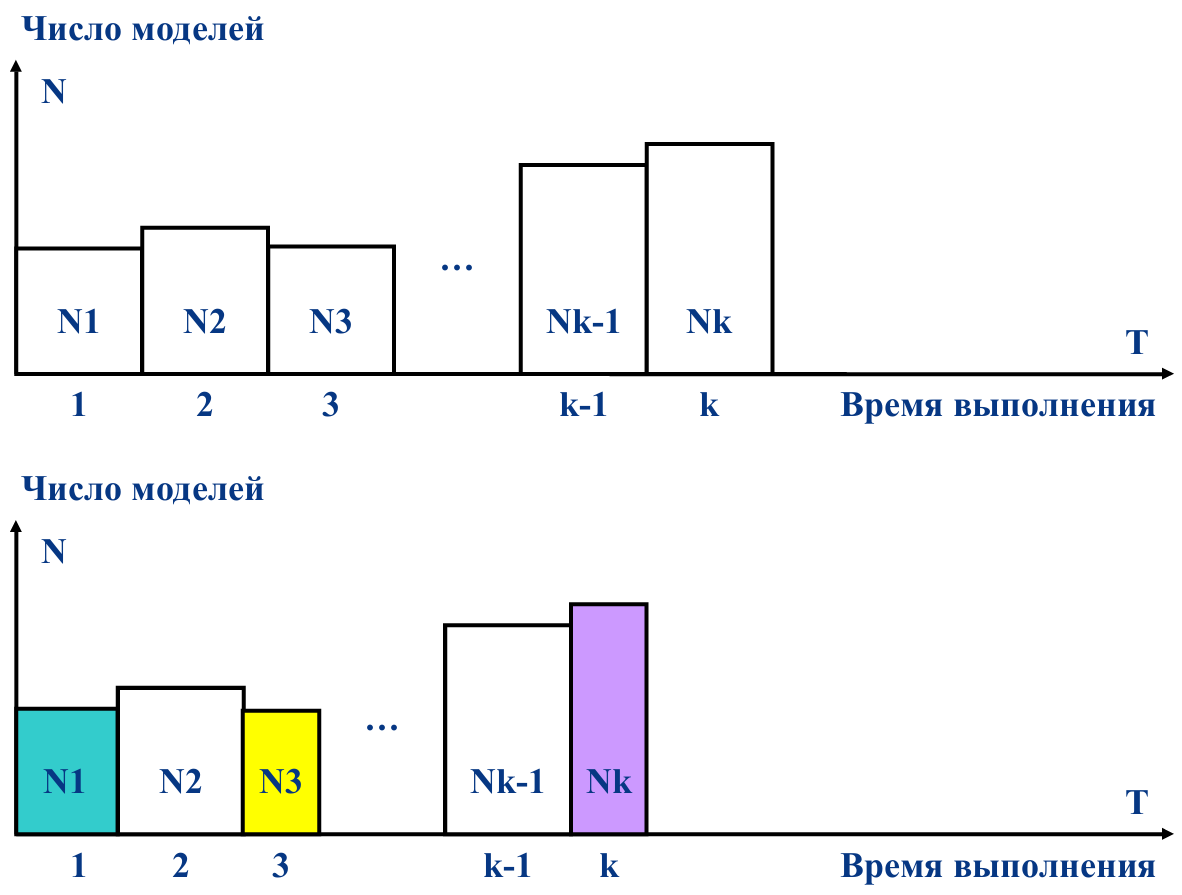
\includegraphics[width=0.8\textwidth]{img/fdiag02.png}
    \caption{Сокращение премени выполнения работ за счет формализации моделей}
    \label{fdiag02}
\end{figure}

Разработка алгоритмов преобразования одних моделей в другие позволяет автоматизировать процесс и обеспечить представление исходной задачи в виде формализованных данных или программы на специализированном (про\-блем\-но--ориентированном или предметно--ориентированном) языке программирования. Фактически это означает слияние моделей задачи и исполнителя (рисунок~\ref{fig01-03b}).

\begin{figure}[htbp]
    \centering
    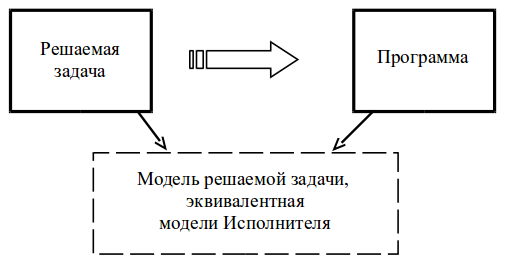
\includegraphics[width=0.7\textwidth]{img/fig01-03b.png}
    \caption{Разработка системы программирования, соответствующей предметной области ведет к непосредственному описанию решаемой задаче и слиянию моделей}
    \label{fig01-03b}
\end{figure}

По такой схеме разрабатываются различные предметно-ориентированные и специализированные языки, а также соответствующи системы программирования. К ним, в частности, можно отнести:

многие языки имитационного моделирования, обеспечивающие непосредсвенное описание моделей (можно отметить такие языки как GPSS, AnyLogic и другие);

системы автоматизированной генерации лексических и синтаксических анализаторов языков программирования по описанию синтаксиса на соответствующих метаязыках (начиная от таких первопроходцев как lex и yacc);

языки международного стандарта IEC 61131-3, ориентированные на разработку ПО логических контроллеров.

В этом случае временные характеристики процесса разработки можно представит в виде исходных моделей предметной области и моделей виртуального исполнителя, программируемого на специализированном или проблемно-ориентированном языке (рисунок~\ref{fdiag03}).

\begin{figure}[htbp]
    \centering
    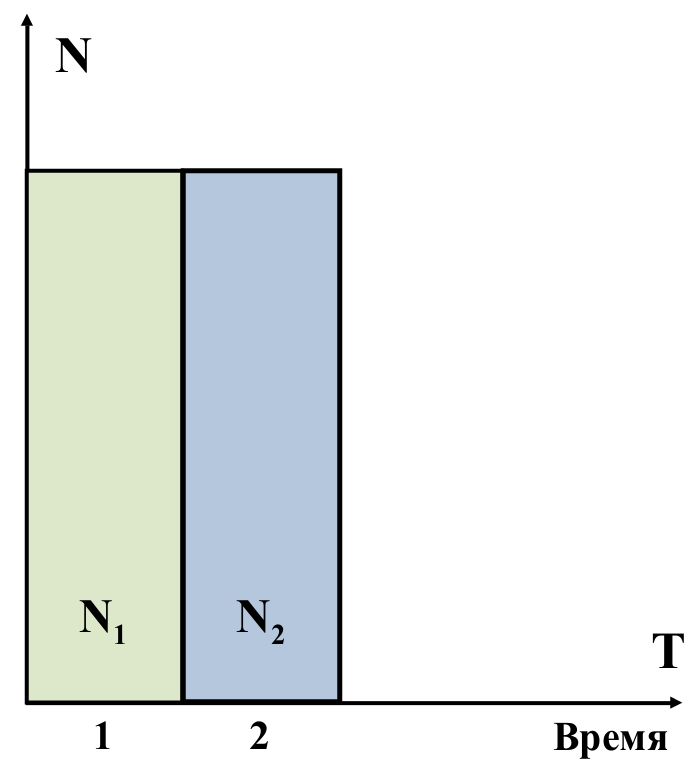
\includegraphics[width=0.4\textwidth]{img/fdiag03.png}
    \caption{Использование специализированного языка для описания моделей предметной области (идеализированный вариант)}
    \label{fdiag03}
\end{figure}

Следует отметить, что помимо языков и специальных сред разработки проблемная ориентация, а следовательно и определенная формализация предметной области, осуществляется за счет использования библиотек в рамках различных универсальных языков программирования. В частности следует отметить разнообразные библиотеки, повышающие эффективность разработки компьютерных игр.

Достоинства подхода, опирающегося на формализацию предметной области, проявляются в следующем:

\begin{itemize}
    \item достижение более высокой скорости разработки программ (к программированию можно приступать уже во время анализа решаемой задачи);
    \item разработкой могут заниматься специалисты-предметники, не являющиеся профессионалами в программировании;
    \item программирование может протекать непосредственно в терминах предметной области, что еще больше повышает эффективность процесса разработки (программирование без программирования).
\end{itemize}


К недостаткам подхода следует отнести:

\begin{itemize}
    \item отсутствие гибкости (предметная ориентация моделей не позволяет непосредственно использовать накопленные методы и инструменты в других областях);
    \item ориентацию на достаточно узкую категорию задач;
    \item необходимость разработки и использования специализированных инструментальных средств.
\end{itemize}

Прием эффективен при решении достаточно простых задач узкого класса, так как увеличение размерности резко повышает количество применяемых специализированных моделей, пригодных для использования в разнообразных предметных областях. Это ведет к увеличению сложности методов формализации и уменьшению эффективности комплексного использования специализированных моделей.

С формализацией предметной области достаточно тесно связан предметно-ориентированный подход к проектированию (Domain--driven design, DDD). Эта связь проявляется в более внимательном изучении контекста прикладной области, выделении в ней различных факторов, для которых можно обеспечить построение более строгих моделей, поддающихся дальнейшей формализации. Наряду с этим в ходе такого проектирования часто формируется язык предметной области, который может быть реализован либо с использованием средств существующих языков программирования, либо путем создания соответствующего специализированного или предметно-ориентированного языка.

В заметке «Формализация предметной области на примере вычисления 100!» представлен простой пример, демонстрирующий специфику данного методического приема.

\subsubsection*{Создание методик разработки программного обеспечения}

Методики разработки программного обеспечения ориентированы на формализацию взаимосвязей между моделями конкретных исполнителей и моделями, используемыми на предшествующих этапах разработки (например, при анализе и проектировании). Место методик (состоящих из набора методов преобразования между различными группами моделей) в процессе разработки ПО представлено на рисунке~\ref{fig01-04}.

\begin{figure}[htbp]
    \centering
    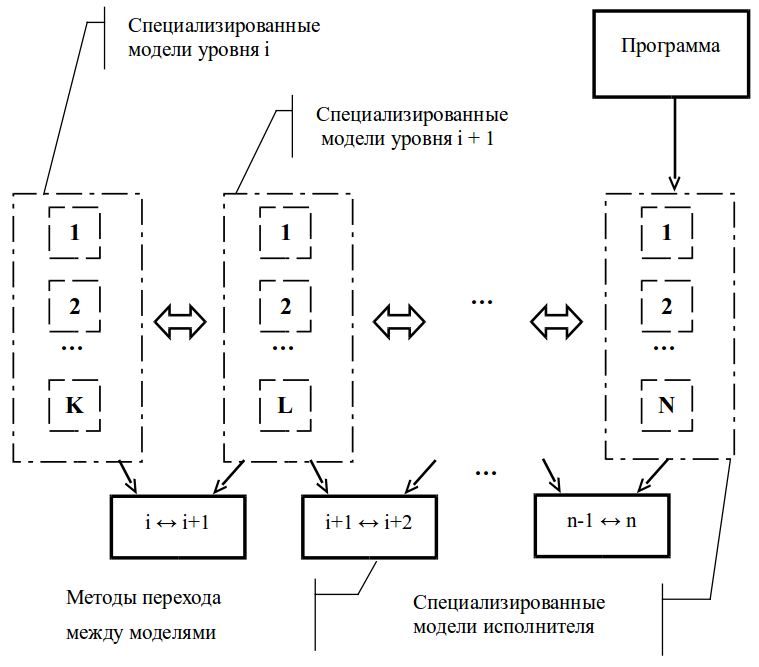
\includegraphics[width=0.9\textwidth]{img/fig01-04.png}
    \caption{Использование методик разработки для поэтапного преобразования моделей}
    \label{fig01-04}
\end{figure}

Изначальная ориентация Исполнителя на универсальность вычислений обычно предполагает применение методик для широкого класса задач, не связывая их непосредственно с предметными областями. Они поддерживают взаимодействие моделей, используемых в разработке, определяя процесс преобразования как от модели задачи к модели исполнителя, так и в обратном направлении.

Несмотря на обеспечение прямого и обратного проектирования, основное достоинство методик проявляется в поддержке нисходящей разработки, что во многом обуславливается большей наглядностью переходов от универсальных высокоуровневых моделей предметных областей к моделям, описывающим соответствующих исполнителей. В подобной ситуации знание задачи повышает эффективность разработки. Поэтому, создание программного обеспечения обычно начинается с привязки модели предметной области к моделям анализа и проектирования, предлагаемым используемой методикой (рисунок~\ref{fig01-05}).

\begin{figure}[htbp]
    \centering
    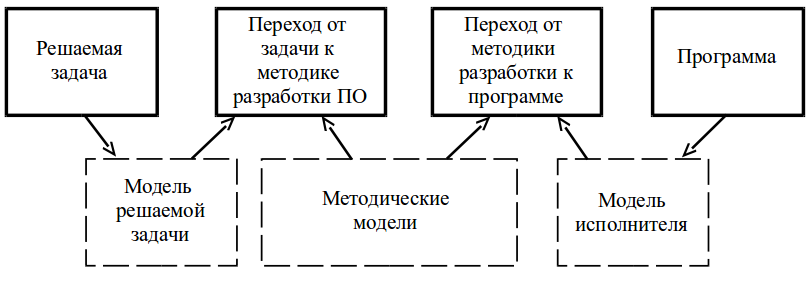
\includegraphics[width=0.9\textwidth]{img/fig01-05.png}
    \caption{Использование методик разработки в виде методических моделей}
    \label{fig01-05}
\end{figure}

Применение методических моделй не влияет непосредственно на скорость разработки специализированных моделей. Однако это позволяет сократить время переходов между различными взаимозависимыми моделями, что в конце концов можно трактовать как сокращение времени перехода между различными этапами процесса разработки. Условно это сокращение показано на рисунке~\ref{fdiag04}.

\begin{figure}[htbp]
    \centering
    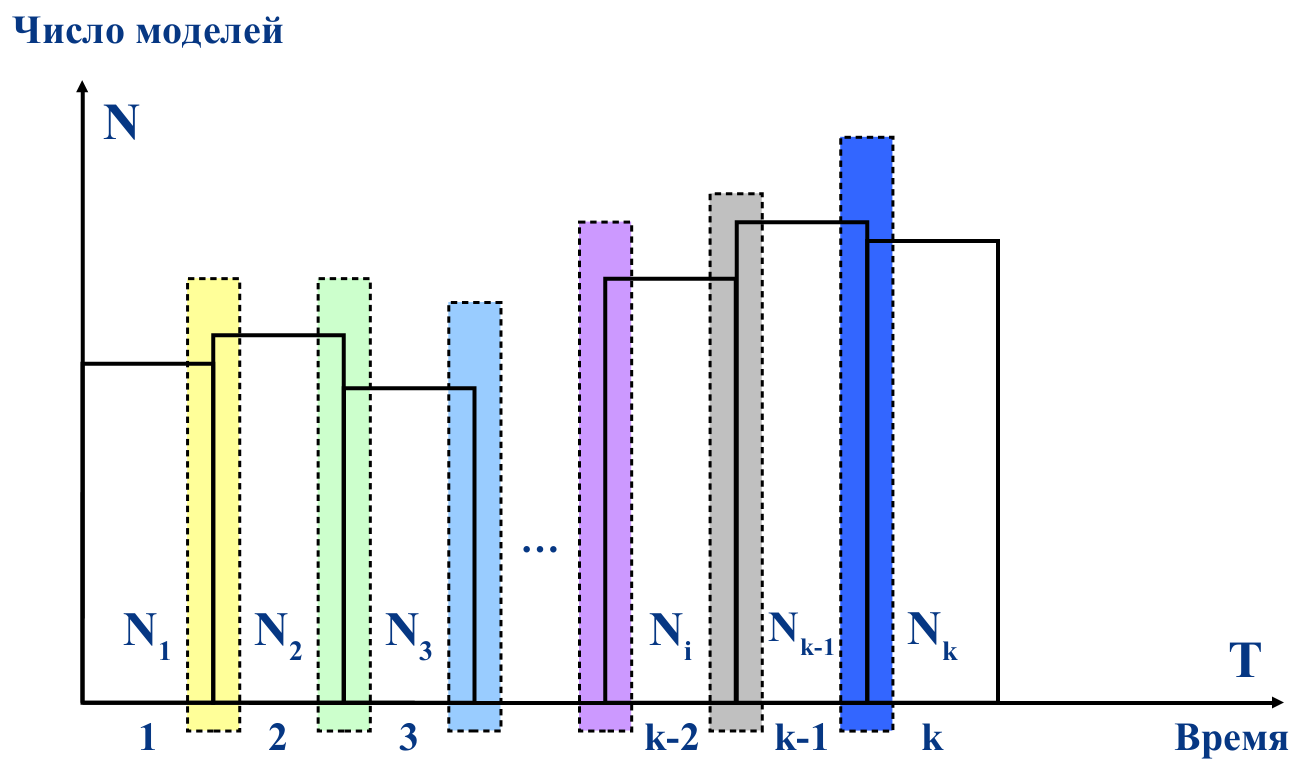
\includegraphics[width=0.9\textwidth]{img/fdiag04.png}
    \caption{Сокращение времени разработки ПО за счет использования методических моделей}
    \label{fdiag04}
\end{figure}

К достоинствам методик разработки ПО следует отнести:

\begin{itemize}
    \item универсальность, что позволяет ориентироваться на разработку задач широкого класса;
    \item поддержку нисходящего и восходящего проектирования;
    \item поддержку прямого и обратного проектирования;
    \item возможность использовать инструментальные средства.
\end{itemize}
К недостатку отдельных методик относится привязка процесса разработки к определенным методам и исполнителям.

В настоящее время существуют различные методики. Они являются составной и неотъемлемой частью методологий разработки программного обеспечения, которые, наряду с процессами создания программ, дополнительно регламентируют организационную деятельность, анализ, тестирование и сопровождение, что в целом определяет организацию жизненного цикла программы на основе единого концептуального подхода. Примерами подобных методик могут служить:

\begin{itemize}
    \item объектно-ориентированный подход, используемый в составе объектно-ориентированной методологии;
    \item методы структурного анализа и проектирования (structured analysis and design technique, SADT), часто применяемые при разработке информационных систем;
    \item методы быстрой разработки приложений (rapid application development, RAD), ориентированные на ускоренное построение программ от моделей, определяющих взаимодействие системы с пользователем.
\end{itemize}

Методики широко используются при разработке больших программных систем, так как повышают эффективность проектирования за счет предоставления достаточно простых и ясных подходов, выработанных на основе эмпирического опыта и теоретических исследований. Их использование, в сочетании с инструментальной поддержкой, обеспечивает сокращение семантического разрыва между моделями задач и исполнителем.

\subsection{Технические приемы}

Технические приемы ориентированы на использование инструментальных средств, поддерживающих различные аспекты процесса разработки ПО. Можно выделить:

\begin{itemize}
    \item средства поддержки методических приемов;
    \item вспомогательные средства;
    \item системы программирования.
\end{itemize}

\subsection*{Поддержка методических приемов}

Инструментальные средства, обеспечивающие поддержку методических приемов, предназначены для компьютерного представления и анализа разрабатываемых моделей, преобразования построенных моделей в другие модели, автоматизации процесса построения требуемой документации, а также ведения организационной деятельности в ходе разработки ПО. Повышая эффективность процесса разработки, средства поддержки методических приемов, в то же время, не определяют сам процесс создания программы. Их использование предполагает дальнейшую доводку программ с применением инструментов, имеющих более тесную связь с архитектурами вычислительных систем.

Примерами ранних средств подобного рода могут служить системы поддержки спецификаций. Во многих из них использовались графические языки, которые в основном играли роль вспомогательного документа. Для написания программы необходимо было вручную осуществлять перевод этих диаграмм в код. Положение изменилось с внедрением CASE-средств. Разработанные инструменты сгладили семантический разрыв между рядом моделей предметной области и кодом, обеспечив непосредственное преобразование, как в прямом, так и в обратном направлении. К средствам поддержки методов структурного анализа и проектирования можно отнести, например, различные системы, обеспечивающие инструментальную поддержку UML, и, следовательно, объектно-ориентированную и другие методологии.

\subsubsection{Вспомогательные средства}

Вспомогательные средства предназначены для повышения эффективности процессов, не связанных с непосредственной разработкой структуры программы, но, в то же время, сильно влияющих на качество и время разработки. К ним следует отнести:

\begin{itemize}
    \item средства отладки программ;
    \item системы тестирования;
    \item средства профилирования и другие.
\end{itemize}

Их специфика заключается в работе с уже готовыми программами, что позволяет считать их влияние на процесс разработки программ косвенным образом.

Отладка используется для локализации и устранения ошибок в разрабатываемых программах. Существуют различные подходы к решению этой задачи. В частности проводятся следующие мероприятия:

\begin{itemize}
    \item анализируются текущие значения различных переменных;
    \item определяются траектории выполнения программы.
\end{itemize}


Эти задачи можно решать путем вставки к исходные тексты программ специальных вспомогательных операторов. Однако вместо этого часто используются специальные отладчики, которые повышают эффективность процесса отладки за счет дополнительных сервисных функций. Отладчики могут использоваться независимо от других инструментальных средств. Примером такого подхода является отладчик gdb. Однако зачастую отладчики непосредственно встраиваются в интегрированные среды разработки программ, что обеспечивает большую наглядность и оперативное исправление возникающих ошибок. К системам, ориентированным на такой подход можно отнести MS Visual Studio. Помимо этого, для повышения эффективности использования автономных отладчиков применяются дополнительные обертки в виде графических интерфейсов (например программа Data Display Debugger (ddd) формирует графический интерфейс вокруг отладчика gdb). Такие обертки могут также встраиваться и в интегрированные среды разработки, позволяя использовать один и тот же отладчик как автономно, так и внутри себя. В качестве примера такой среды можно выделить Qt Creator.

Тестирование заключается в проверке соответствия между реальным и ожидаемым поведением программы. Осуществляется на наборе тестов, подобранном определенным образом. Существуют разнообразные методы тестирования, которые обуславливаются особенностями процесса разработки программ на различных этапах. Это, в свою очередь, ведет к применению широкого набора разнообразных инструментальных средств, повышающих эффективность процесса разработки. Помимо этого тестирование может определять организацию процесса программирования, если используются методы разработки через тестирование (Test Driven Development — TDD).

Профилирование направлено на сбор и анализ характеристик, определяющих особенности функционирования программы. К ним относятся: время выполнения отдельных фрагментов кода (подпрограмм, функций, потоков, процессов), количество истинных и ложных переходов в различных условных операторах и операторах цикла, количество кэш промахов и т. д. Инструмент, предназначенный для получения этих характеристик, называется профилировщиком. Полученные данные используются для оптимизации программы повышающей эффективность ее функционирования, которая обычно связана с улучшением таких критериев качества как уменьшение времени выполнения программы, уменьшение объема занимаемой памяти и рядом других характеристик.

\subsubsection{Системы программирования}

Системы программирования – это инструментальные средства, поддерживающие разработку программ для заданного виртуального исполнителя и их последующее автоматическое преобразование в программы реального исполнителя.

Использование систем программирования позволяет решать задачу повышения эффективности процесса разработки ПО за счет сокрытия исполнителей более низкого уровня, являющихся реальными вычислительными системами (рисунок~\ref{fdiag05}). Такой подход широко используется на практике и позволяет писать программы для высокоуровневого исполнителя (определяемого часто как архитектура виртуальной машины).

\begin{figure}[htbp]
    \centering
    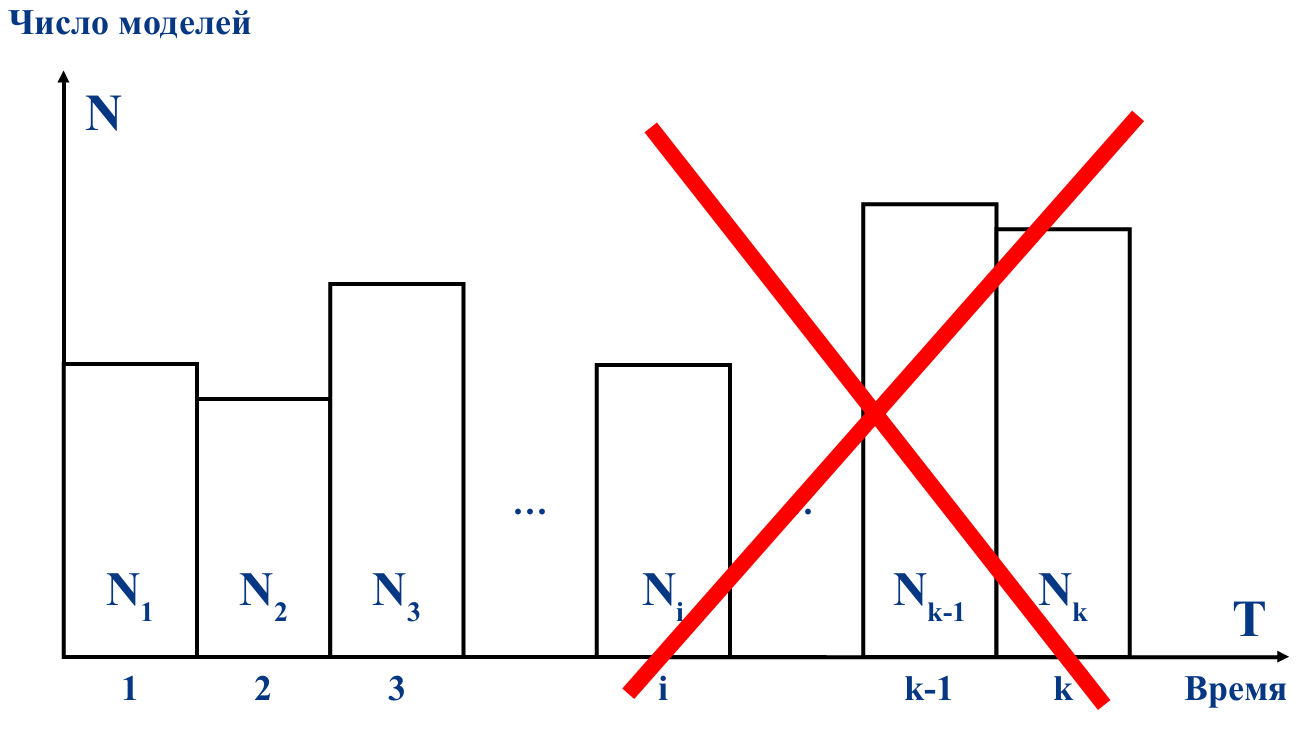
\includegraphics[width=0.9\textwidth]{img/fdiag05.png}
    \caption{Системы программирования «убирают» часть моделей из процесса разработки}
    \label{fdiag05}
\end{figure}


Выполнение полученных программ может осуществляться:

\begin{enumerate}
    \item Использованием непосредственной интерпретации, полностью скрывающей процесс реального выполнения, который может оказаться намного сложнее. Схема, иллюстрирующая подход, представлена на рисунке~\ref{fig01-06}.
\begin{figure}[htbp]
    \centering
    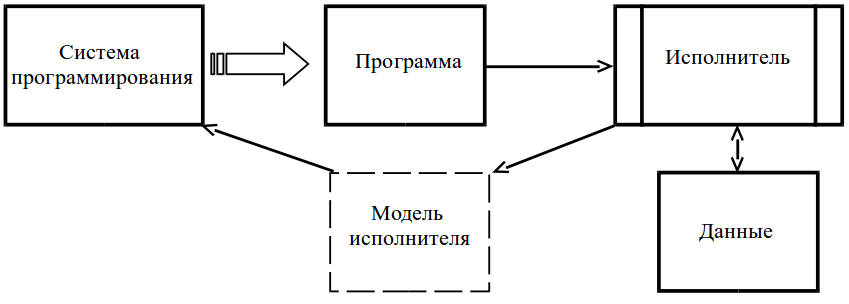
\includegraphics[width=0.9\textwidth]{img/fig01-06.png}
    \caption{Непосредственное использование исполнителем программы, написанной с применением системы программирования}
    \label{fig01-06}
\end{figure}
    \item Автоматическим и поэтапным преобразованием программы, написанной для виртуальной машины, в программу конечного исполнителя, обеспечивающего ее интерпретацию, что позволяет разрабатывать программы для систем, не допускающих непосредственное выполнение. Подобный прием применяется, например, в системах компиляции. Возможен вариант, когда преобразование программы является многоступенчатым, что может оказаться целесообразным при использовании нескольких промежуточных моделей исполнителей. Схема преобразований приведена на рисунке~\ref{fig01-07}. Проводимые промежуточные преобразования могут быть скрыты от программиста. Однако дополнительные знания о конечном исполнителе позволяют повысить эффективность процессов отладки и выполнения программы.
\end{enumerate}

\begin{figure}[htbp]
    \centering
    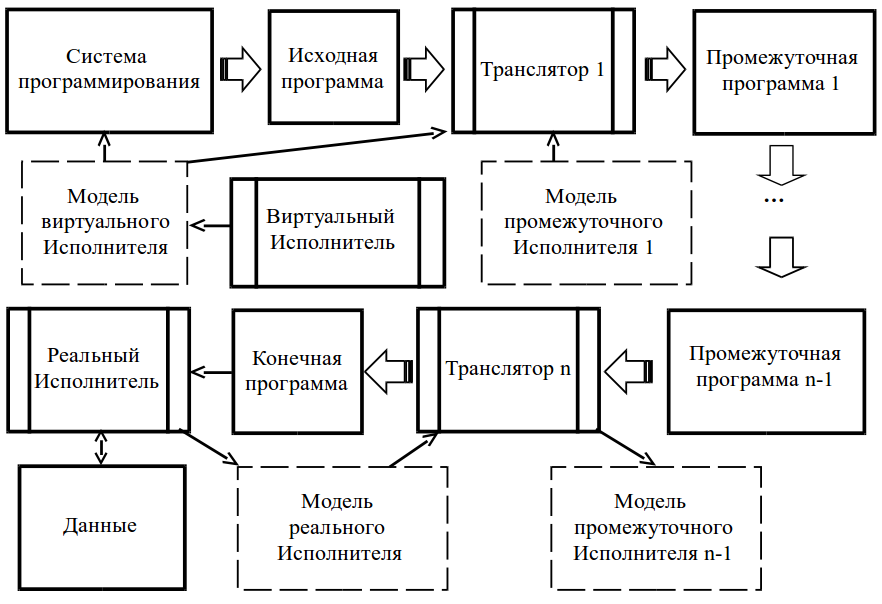
\includegraphics[width=0.9\textwidth]{img/fig01-07.png}
    \caption{Многоэтапное преобразование модели исполнителя, поддерживаемого системой программирования, в модель исполнителя, реально осуществляющего вычисления}
    \label{fig01-07}
\end{figure}

Каждый из представленных подходов может использовать одно и то же исходное представление программы. Их отличие проявляется на уровне дополнительных сервисов и знаний о моделях, применяемых в цепочке преобразований от исходного исполнителя до интерпретатора. В целом процесс работы конечного исполнителя не является определяющим для процесса разработки исходной программы.

Исполнители могут отличаться и по степени приближения их моделей к моделям решаемых задач или более высокоуровневым методологическим моделям. Использование в их архитектуре моделей решаемых задач ведет к разработке специализированных и проблемно-ориентированных систем программирования. Ориентация на общие модели проектирования обуславливает создание высокоуровневых универсальных средств. При ориентации на архитектуры реальных вычислительных систем можно разрабатывать более производительные программы. Однако процесс разработки усложняется за счет дополнительной детализации.


subsection{Связь между различными моделями процесса разработки и рассмотренной схемой}

В принципе представленный в заметке модельный взгляд отличается от существующих моделей жизненного цикла процесса разработки ПО только акцентом на другие параметры. Если рассматривать существующие подходы и классификации, то в них основное внимание уделяется этапам, а не их содержанию (речь идет о схемах, а не их детализации). В частности, в представленной на рисунке~\ref{fdiag06} водопадной модели четко выделены основные этапы процесса разработки, с каждым из которых связан свой комплекс работ и распределение ролей.

\begin{figure}[htbp]
    \centering
    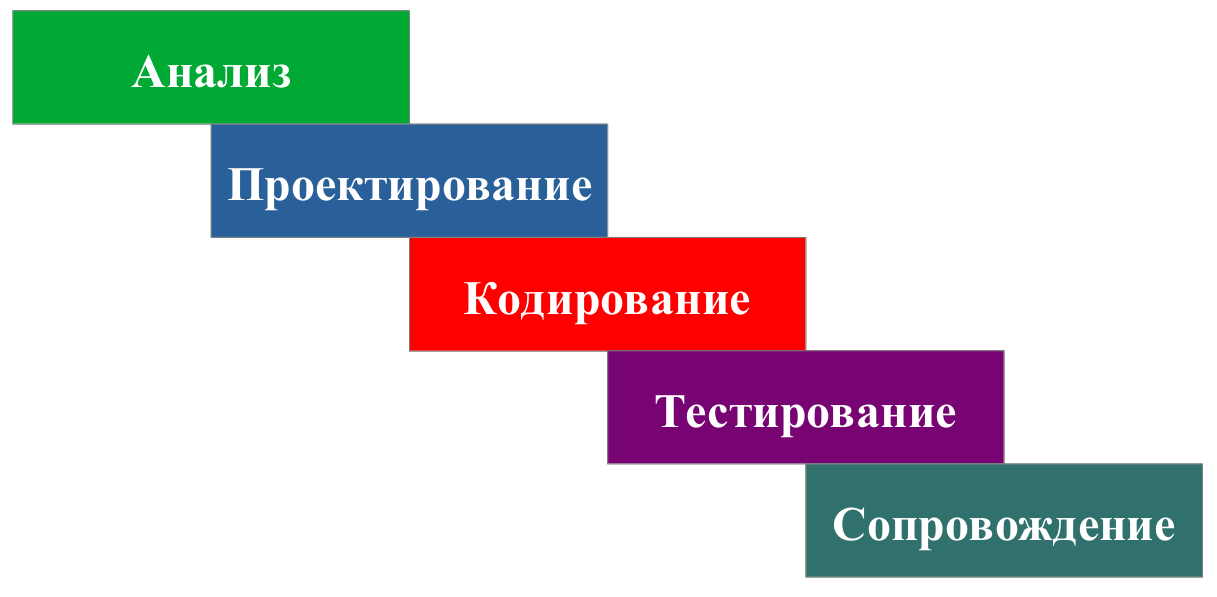
\includegraphics[width=0.9\textwidth]{img/fdiag06.png}
    \caption{Водопадная (каскадная) модель разработки ПО}
    \label{fdiag06}
\end{figure}

Ничто не мешает осуществить поэтапное разпределение и для специализированных моделей (рисунок~\ref{fdiag07}). Однако следует заметить, что и при этом основной упор в дальнейшей детализации будет направлен на характеристики моделей, а распределение работ между исполнителями будет связано не только с их разделением по этапам, но и с назначением им специализированных моделей внутри каждого из этапов.

\begin{figure}[htbp]
    \centering
    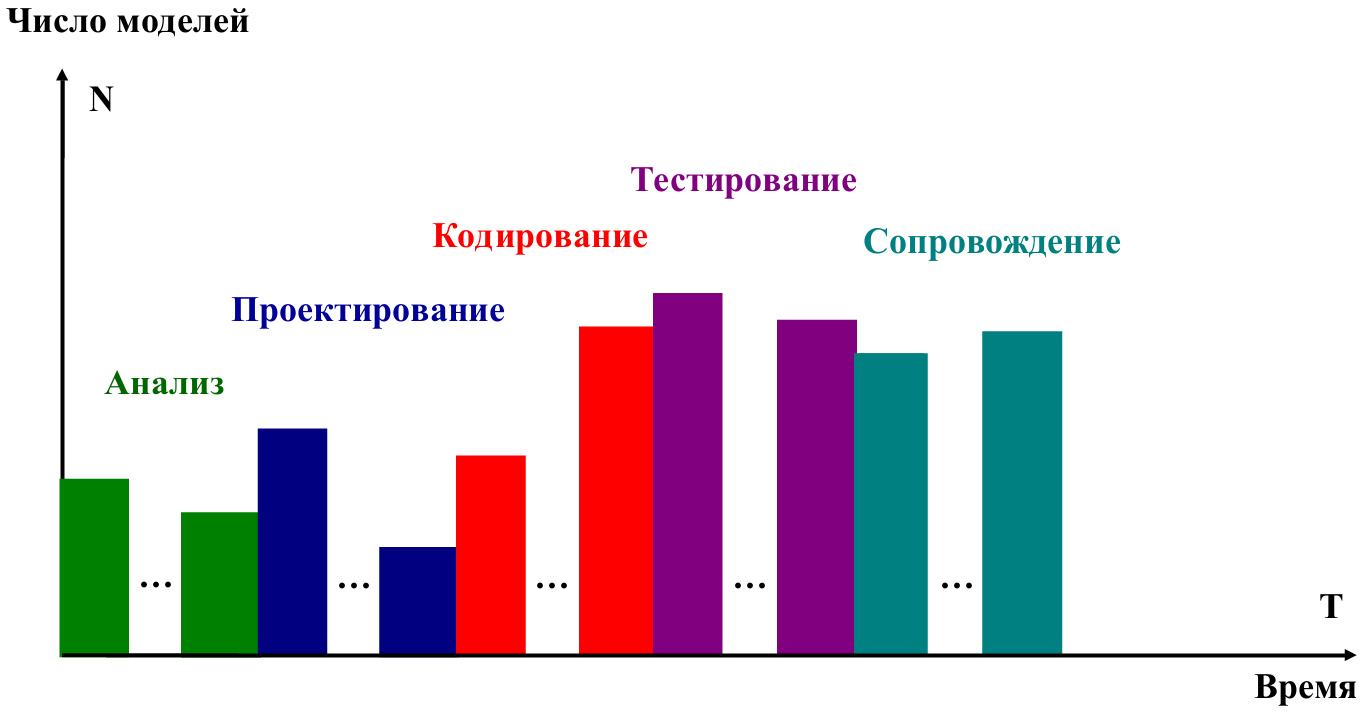
\includegraphics[width=1.0\textwidth]{img/fdiag07.png}
    \caption{Связь с водопадной моделью разработки ПО}
    \label{fdiag07}
\end{figure}

Аналогичным образом можно интерпретировать и итерационную (возвратную, спиральную) модель (рисунок~\ref{fdiag08}). Каждая очередная итерация заключается в повторении этапов разработки на каждом из которых выполняется расширение функциональности программного продукта.

\begin{figure}[htbp]
    \centering
    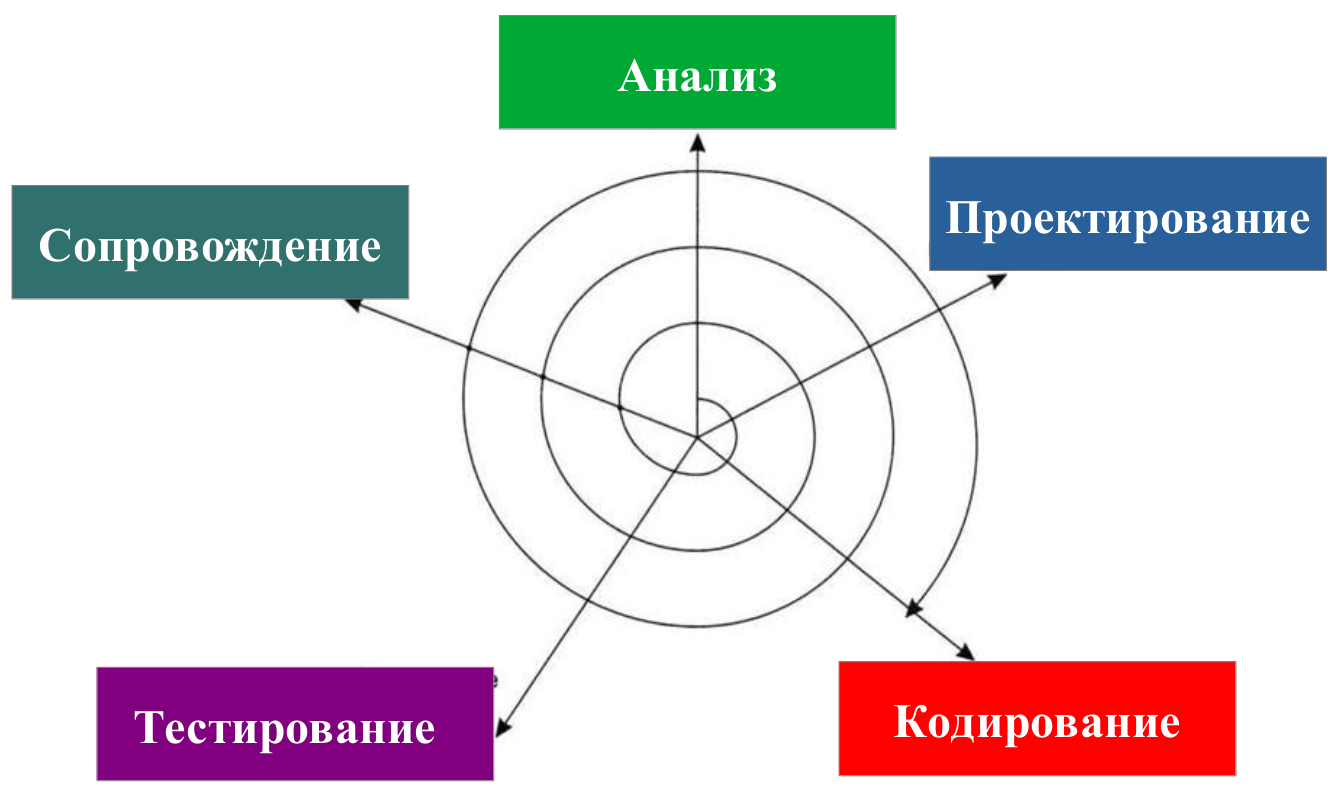
\includegraphics[width=1.0\textwidth]{img/fdiag08.png}
    \caption{Итерационная (возвратная) модель разработки ПО}
    \label{fdiag08}
\end{figure}

Это расширение можно интерпретировать как разработка только части моделей, распределенных по каждому из этапов (рисунок~\ref{fdiag09}). Помимо этого в модельной интерпретации можно также фиксировать зависимости между моделями отдельно для каждого витка итерации, стремясь при этом к тому, чтобы зависимости между моделями разных итераций были как можно меньше. Это ведет к тому, что планирование итераций на уровне специализированных моделей может дополнительно включать учет зависимостей между ними.

\begin{figure}[htbp]
    \centering
    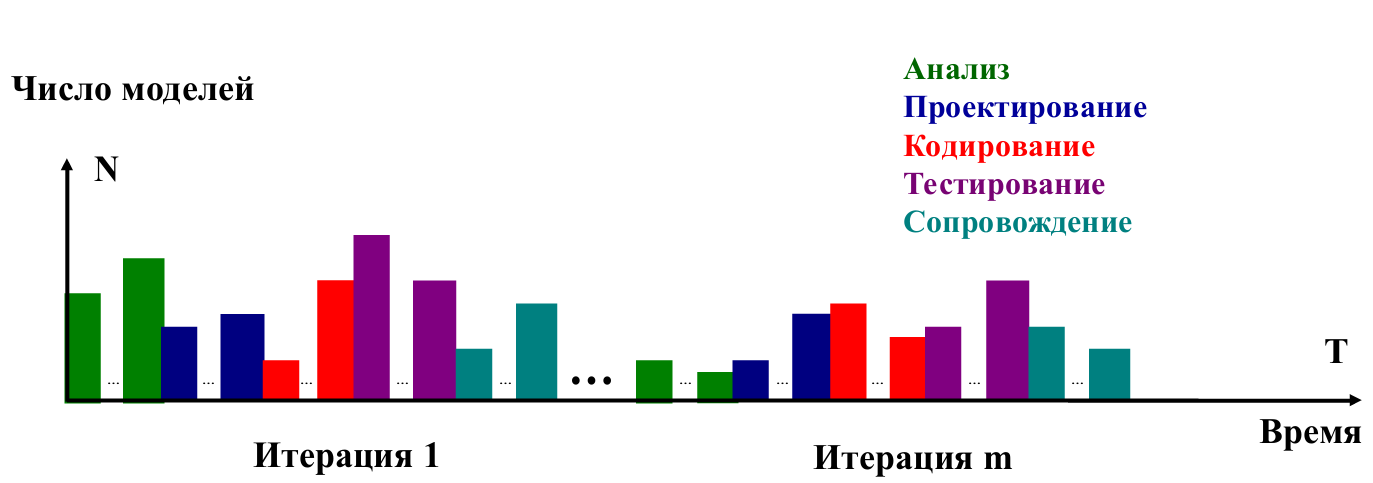
\includegraphics[width=0.9\textwidth]{img/fdiag09.png}
    \caption{Связь с итерационной моделью разработки ПО}
    \label{fdiag09}
\end{figure}

В целом следует отметить, что аналогичным образом можно взгляд модельный взгляд можно накладывать на различные модификации двух основны (рассмотренных выше) процессов разработки. Помимо этого в целом процесс разработки можно интерпретировать и независимо от этапов, акцентируя при этом внимание на определении специализированных моделей и установлении зависимостей между ними. На основании этого можно применять для процесса разработки ПО более гибкое планирование ресурсов и разработчиков.

\subsection{Выводы}

Рассмотрены основные понятия, связанные с процессом разработки программного обеспечения. Разработка программ непосредственно связана с использованием моделей, обеспечивающих описание решаемой задачи, применяемого исполнителя, промежуточных преобразований модели решаемой задачи в модель исполнителя. При этом между моделями решаемой задачи и моделями исполнителя существует семантический разрыв, преодоление которого осуществляется с использованием методологических и технических приемов, разнообразие которых определяется множеством различных факторов. Множество специализированных моделей может формироваться в зависимости от различных факторов. Повышение эффективности процесса разработки ПО во многом обеспечивается использованием соответствующих инструментальных средств.

\subsection{Вопросы}

\begin{enumerate}
    \item Опишите известную Вам предметную область. Какие модели необходимо задать для ее описания перед переходом к разработке программного продукта.
    \item Приведите характеристики компьютерных архитектур, используемых для выполнения программного обеспечения в известной Вам предметной области.
    \item Как проявляется семантический разрыв при разработке программного обеспечения? Какие существуют подходы для его сокращения?
    \item Приведите примеры известных Вам предметных областей, в которых применяютс методы формализаци.
    \item Какие из известных Вам методов формализации реализованы в виде систем или языков программирования?
    \item Приведите примеры предметно-ориентированных или специализированных языков, ориентированных на какую-либо предметную область. Как в этих языках отражается формализация предметной области?
    \item Приведите примеры библиотек, ориентированных на разработку компьютерных игр. На каких языках программирования написаны эти библиотеки? Какие языки программирования они поддерживают?
    \item К каком виду методических приемов относятся паттерны проектирования?
    \item Приведите примеры известных Вам инструментальных средств, обеспечивающих техническую поддержку методических приемов.
    \item Приведите примеры специализированных моделей, которые можно было бы сопоставить с различными этапами водпадного (каскадного) проектирования.
    \item Наряду с водопадной и итерационной моделями разработки существуют различные их модификации. Приведите примеры таких моделей и опишите их особенности.
\end{enumerate}


